% !TEX root = dissertation.tex

%
% phdtex
%
% Copyright (c) 2014-2017, Andrew Kanner <andrew.kanner@gmail.com>.
% All rights reserved.
%
% SPDX-License-Identifier: CC-BY-4.0
%

\begin{singlespace}
  \realchapter{Название главы 1} \label{chapt1}
\end{singlespace}

% комментарии разработчика шаблона
Для более удобного использования cvs типа git лучше использовать
редактор с переносом строк длиной более 80 символов. Так будет проще
вносить и затем просматривать изменения по длинным абзацам.

Перенос строк в latex не является признаком начала нового абзаца,
новый абзац начинается если перед текстом вставлена пустая строка (как
перед этим предложением). \\

\section{Название раздела 1.1} \label{sect1_1}

Текст раздела \dots{} \\

Нумерованный список:
\begin{enumerate}
\item пункт 1;
\item пункт 2;
\item пункт 3. \\
\end{enumerate}

Ненумерованный список:
\begin{itemize}
\item пункт 1;
\item пункт 2;
\item пункт 3. \\
\end{itemize}

Список c произвольными разделителями:
\begin{description}
\item{\textbf{[п1]}} пункт 1;
\item{\textbf{[п2]}} пункт 2;
\item{\textbf{[п3]}} пункт 3. \\
\end{description}

Совмещенные списки:
\begin{enumerate}
\item пункт 1:
      \begin{itemize}
      \item подпункт 1.
      \end{itemize}
\item пункт 2;
\item пункт 3. \\
\end{enumerate}

Список myenumerate (см. contrib/stylesgost.tex):
\begin{myenumerate}
\item пункт 1;

  Дополнительный длинный-длинный-длинный текст без изменения
  форматирования по отношению к основному тексту вне списка.

\item пункт 2;
\item пункт 3. \\
\end{myenumerate}

Пример рисунка (см. Рисунок \ref{test1}). \\

\begin{figure}[bhtp]
  \centering 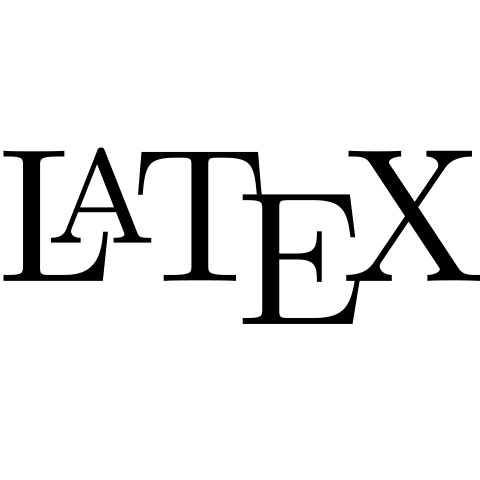
\includegraphics[scale=0.1]{latex-cc0}
  \caption{Подпись рисунка} \label{test1}
\end{figure}

Символ\_подчеркивания, символ процента -- \%. \\

Числа вводятся в math mode: $1$, $2$, $3$ \dots{} \\

Запрет переноса специфических терминов, неразрывный пробел:
\mbox{идентификация/аутентификация} или \mbox{ФСТЭК},
эту~фразу~переносить~нельзя
(только~целиком~или~по~правилам~переносов~слов). \\

Сокращения и условные обозначения: операционная система
(\nom{ОС}{Операционная система}). \\

<<Правильные>> кавычки. Правильное тире --, теперь длинное ---. \\

Выделения текста: \textbf{bold}, \textit{italic},
\underline{underline}, \hly{цветом}, \dots{} \\

Ссылки: литературные источники \cite{article_other}, несколько вместе
\cite{article_pub, article_vak, article_scopus, book1, thesis1,
  conference1, hyperlink1}; сноски\footnote{Текст сноски.}; ссылки на
любые помеченные сущности с помощью label, например на главу
\ref{chapt1}, ссылки на страницу с помеченной сущностью
\pageref{chapt1}. \\

\subsection{Подраздел} \label{subsect1_1_1}

\subsubsection{<<Подподраздел>>} \label{subsect1_1_1_1}

% этот label используется для простановки номеров страниц в Положениях
% из введения
Конец раздела.\label{sect1_1-eof}

%\newpage
%===============================================================================

\section{Название раздела 1.2} \label{sect1_2}

%\newpage
%===============================================================================

\section{Выводы} \label{sect1_3}

\begin{enumerate}
\item Вывод 1.
\item Вывод 2.
\item Вывод 3.
\end{enumerate}

%\clearpage
